\documentclass[../../DD.tex]{subfiles}
\begin{document}
\subsection{Home page}
    The "Home page" (shown in Figure \ref{fig: Home_Page_screenshot}) introduces the company's motto and provides four main sections for user exploration. Users can navigate through two of these sections using two buttons displayed on the top of the homepage. Additionally, by clicking on the "Learn More" button, users can access the "About Us" page to gain a deeper understanding of the company's goals and history.

    The second section of the website highlights the reasons why other companies should choose VenTour. Users can conveniently click on the "Join Us" button to send an email expressing their interest in becoming a part of the company.

    In the third section of the Home Page, which can also be accessed through the buttons at the top of the page, users can explore the global presence of the company and see its worldwide reach.

	%At the beginning of the \textit{Home page} (it can be see in \ref{fig: Home_Page_screenshot}) the motto of the company is presented and the user can browse thanks to two buttons in the two main section of the homepage, but can also click on "Learn More" to go in the page "About us" and better understand what is the goal of the company and what is its history.\\
   %The second section of the website is about the why an other company has to choose VenTour, and the user can easily click on Join Us to send an email in order to ask to be part of the company.\\
    
    %In the third section of the Home Page (also achievable by the buttons in top of the page), the user can see where the company is spread all around the world.\\

	\begin{figure}[!htb]
	    \centering
	    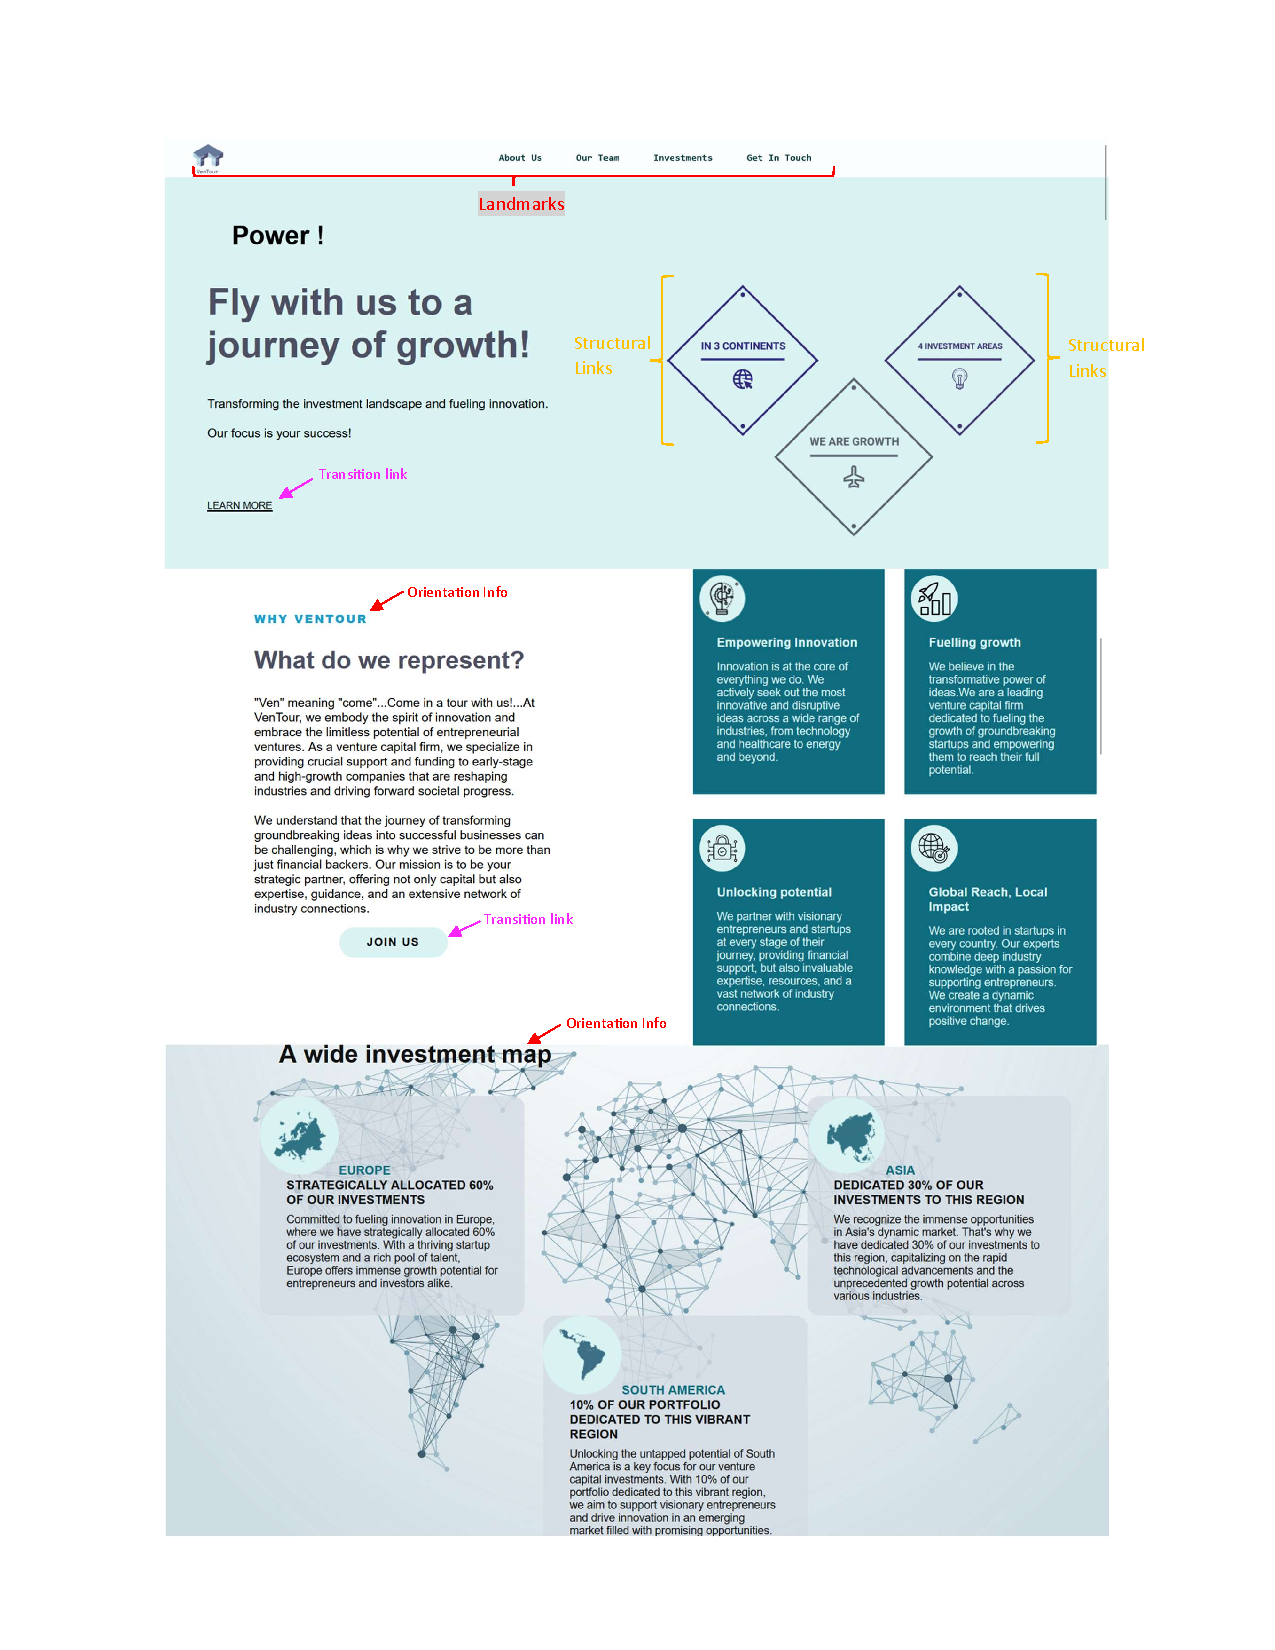
\includegraphics[width=\textwidth]{Images/screenshots/Home Page.pdf}
	    \caption{Home page screenshot}
	    \label{fig: Home_Page_screenshot}
	\end{figure}
    In the fourth and fifth section are shown the 4 top investments and the four areas of investment in which VenTour is specialized.

    \begin{figure}[!htb]
        \centering
        \includegraphics[width=\textwidth, page=2, trim=0 250 0 0, clip]{Images/screenshots/Home Page.pdf}
        \caption{Home page screenshot}
        \label{fig: Home_Page_screenshot2}
    \end{figure}
\end{document}
